\chapter{Aerodinâmica}

\section{Dimensionamento da hélice}

Para o dimensionamento da hélice, inicialmente calculou-se o valor do parâmetro adimensional $j = \frac{V}{nD}$, onde $V$ é a velocidade de cruzeiro, $n$ é a frequência de rotação da hélice e $D$ é o diâmetro. Sabendo que a velocidade da ponta da hélice é dada por
\begin{equation}
V_\text{tip} = \sqrt{(n \pi D)^2+V^2}
\end{equation}
podemos escrever
\begin{equation}
j= \pi\frac{V}{\sqrt{V_\text{tip}-V^2}}
\end{equation}
Considerando que a velocidade da ponta é limitada por perdas de compressibilidade, o número de mach da ponta será limitado a 0,75.

Na condição de cruzeiro, $V=140\si{m/s}$ e a velocidade do som é $a=310\si{m/s}$. O valor de $j$ é então 2,37.

Para obter-se eficiência na faixa de 85\%, selecionou-se uma hélice hexa-pá. De acordo com a \autoref{fig:naca-helice}, a eficiência da hélice para esse valor de $j$ é de 86\% e o coeficiente de tração $T_c = 0,03$. O coeficiente de tração é definido
\begin{equation}
T_c = \frac{\eta P}{\rho D^2 V^3}
\end{equation}
onde $\eta$ é a eficiência da hélice, $P$ é a potência desenvolvida e $D$ é o diâmetro da hélice. Resolvendo essa equação para o diâmetro, temos
\begin{equation}
\label{eqn:D_helice}
D = \sqrt{\frac{\eta P}{\rho V^3 T_c}}
\end{equation}

\begin{figure}[H]
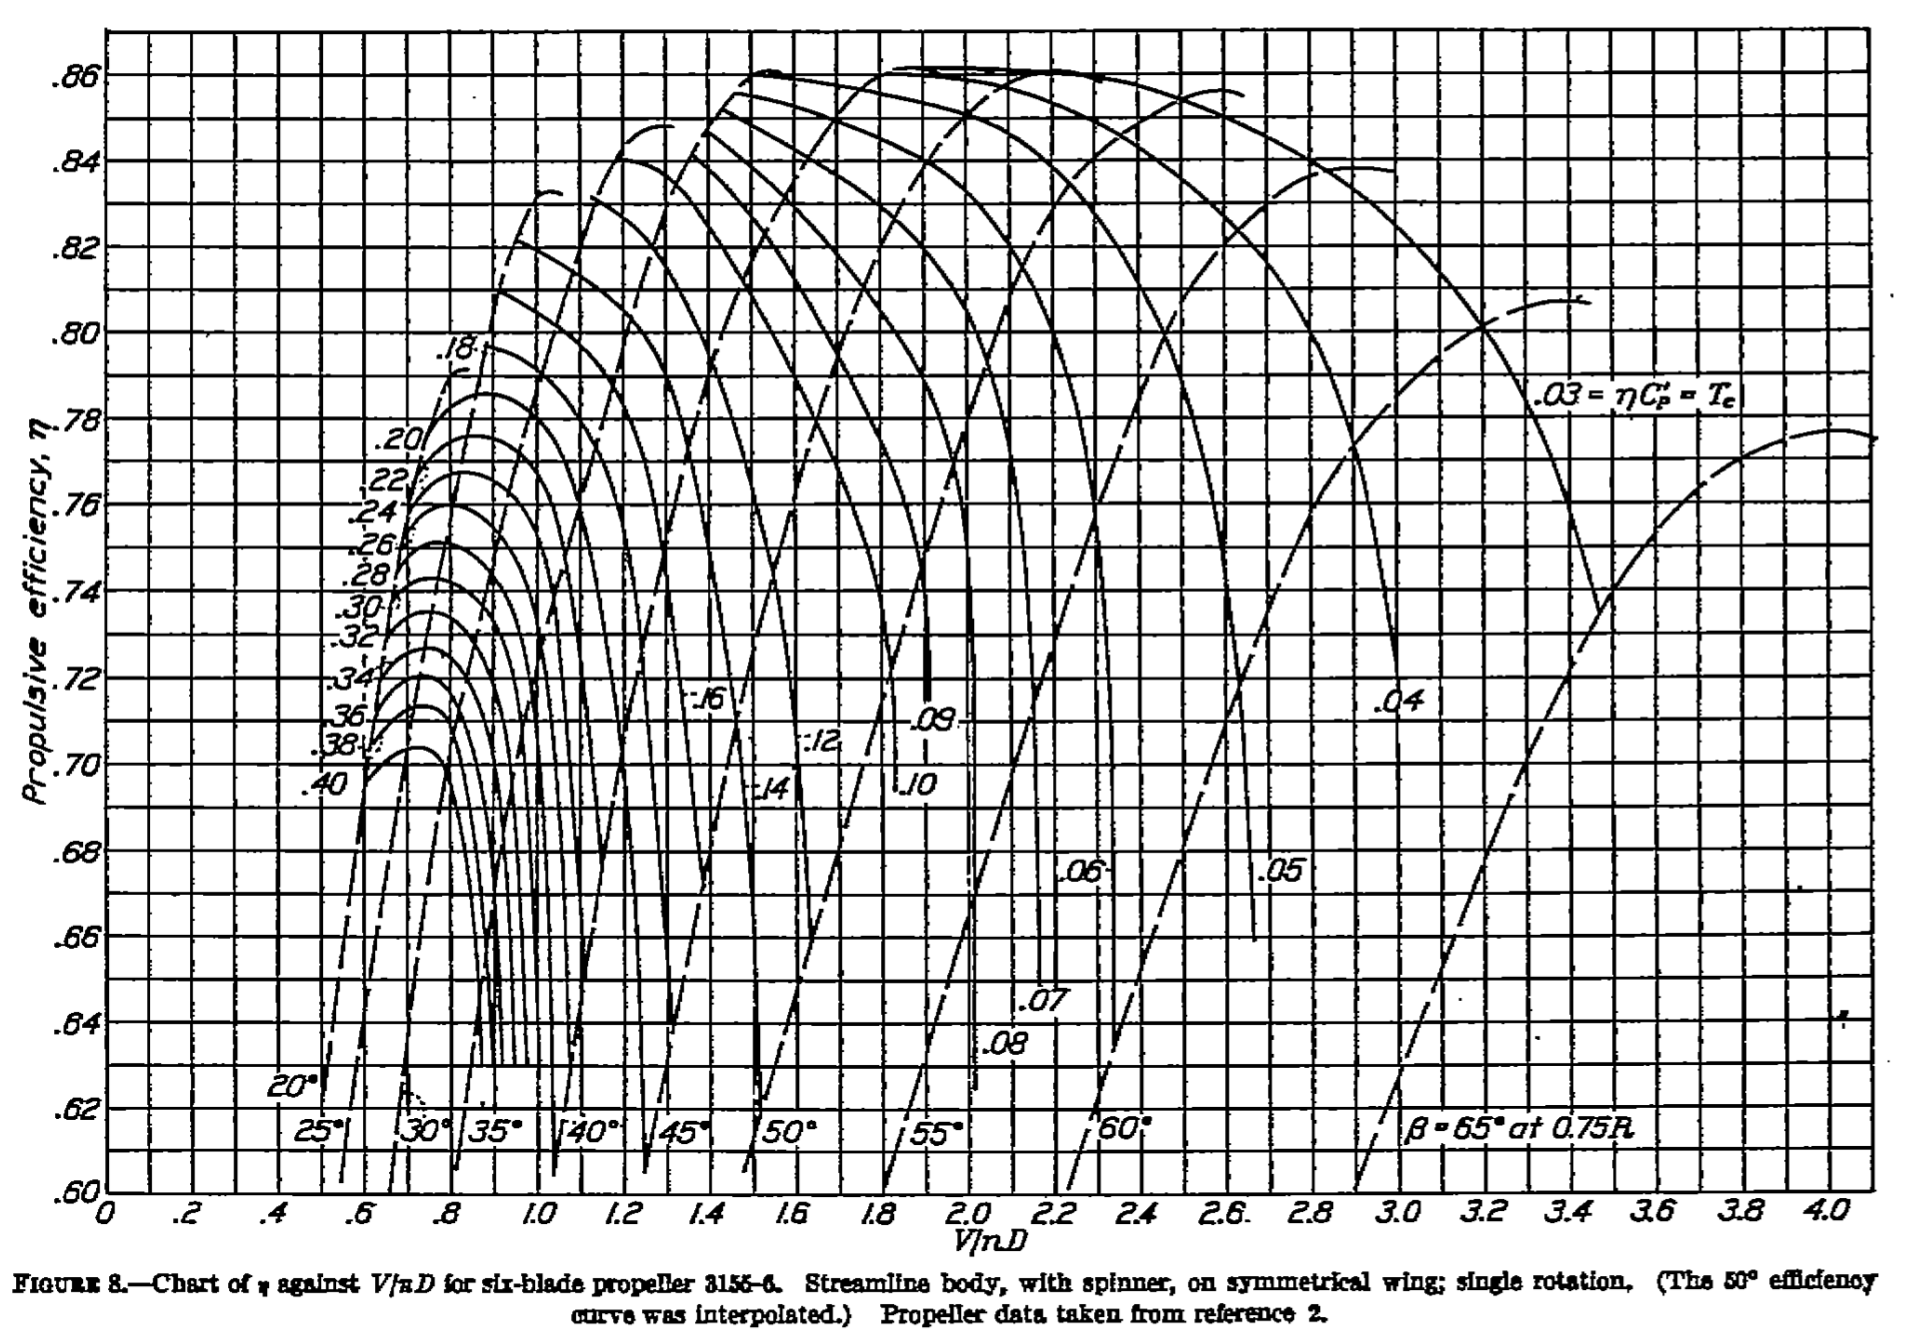
\includegraphics[width=\textwidth]{naca-helice}
\caption{Desempenho de hélice hexa-pá}  % \cite{naca-helice}
\label{fig:naca-helice}
\end{figure}

A potência requerida de decolagem é de 1383\si{kW}, ou seja, 692,5kW por hélice. Substituindo os valores na \autoref{eqn:D_helice}, o diâmetro final fica de
\begin{equation}
D=4,226\si{m}
\end{equation}

Esse diâmetro é aproximadamente duas vezes o diâmetro da fuselagem, de 2,1\si{m}, então não há risco de interferência da hélice com o solo.

%Potencia no cruzeiro: 1383kW (requerida) 2108kW (disponivel) para as duas helices

%Potencia na subida: 3692kW (dimensionante do motor)



\section{Superfícies Sustentadoras}
\label{superf_sustentadoras}

Após a definição do ponto de projeto, forma em planta da asa e das empenagens, realizou-se a modelagem aerodinâmica das superfícies sustentadoras a fim de quantificar a polar de arrasto de cada uma bem como seu $C_{L_{max}}$. Além disso, o cálculo das principais derivadas longitudinais foram determinadas iterativamente com a análise de estabilidade e controle longitudinal visto que as empenagens tiveram suas geometrias refinadas. Utilizou-se os ábacos disponiveis em ETKIN, o software XFOIL para determinação das polares 2D e o software CEA-VLM desenvolvido pelo CEA-UFMG para determinação das polares 3D. As \autoref{superf_sustentadoras,eh,ev} apresentam as curvas $C_L$ x $\alpha$ e as polares de arrasto.

\subsection{Asa}
\label{asa}
A asa foi modelada utilizando o software CEA-VLM. Abaixo tem-se os paineis gerados pelo código em MATLAB para asa.

\begin{figure}[H]
\centering
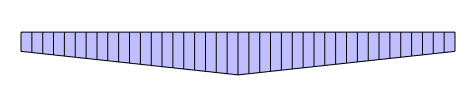
\includegraphics[width=1\textwidth]{images/parte3/malha_asa.PNG}
\caption[Paineis aerodinâmicos - Asa]{Paineis aerodinâmicos - Asa}
\label{fig:malha_asa}
\end{figure}

\begin{figure}[H]
\centering
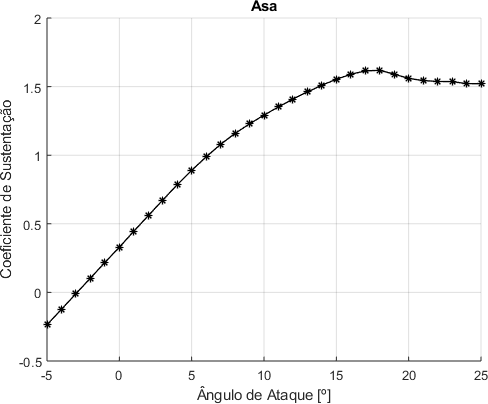
\includegraphics[width=0.75\textwidth]{images/parte3/asa_cl_alfa.png}
\caption[Curva $C_L$ x $\alpha$ para a Asa]{Curva $C_L$ x $\alpha$ para a asa}
\label{fig:asa_cl_alfa}
\end{figure}

\begin{figure}[H]
\centering
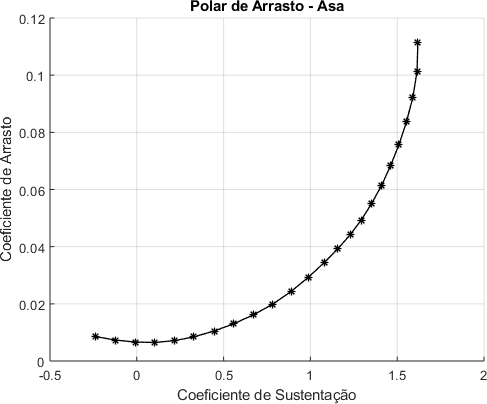
\includegraphics[width=0.75\textwidth]{images/parte3/asa_cl_cd.png}
\caption[Polar de arrasto para a Asa]{Polar de arrasto para a asa}
\label{fig:asa_cl_cd}
\end{figure}

\begin{table}[H]
\centering
\begin{tabular}{cc}
\toprule
$ \frac{\partial C_{l}}{\partial \alpha} $ & 4.740 \\ [0.3cm]
$ \frac{\partial C_{L}}{\partial \alpha} $ & 4.586 \\ [0.3cm]
$ C_{L_{max}} $ & 1.619 \\ [0.3cm]
$ \alpha_{estol} $ & 18\textdegree\ \\ [0.3cm]
$ c_{L_0} $ & 0.3293 \\ [0.3cm]
$ c_{M_0} $ & -0.0447 \\ [0.3cm]
$ c_{M_{\alpha}} $ & 0.3196 \\ [0.3cm]
$ x_{CA}/cma $ & 0.1803 \\ [0.3cm]
\bottomrule
\end{tabular}
\caption[Resultados - Asa]{Resultados - Asa}
\label{tbl:resultados_asa}
\end{table}

\subsection{Empenagem Horizontal}
\label{eh}

\begin{figure}[H]
\centering
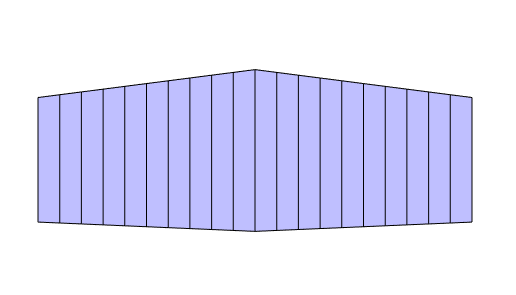
\includegraphics[width=0.45\textwidth]{images/parte3/malha_eh.PNG}
\caption[Paineis aerodinâmicos - Empenagem Horizontal]{Paineis aerodinâmicos - Empenagem Horizontal}
\label{fig:malha_eh}
\end{figure}

\begin{figure}[H]
\centering
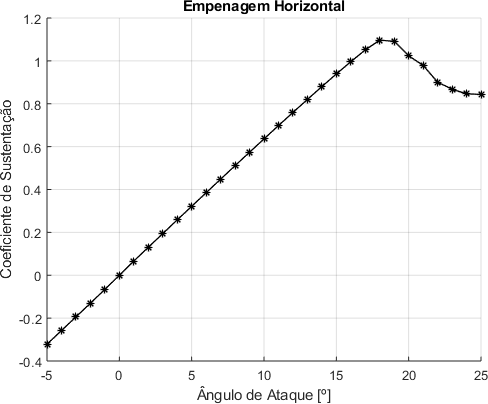
\includegraphics[width=0.75\textwidth]{images/parte3/eh_cl_alfa.png}
\caption[Curva $C_L$ x $\alpha$ para a Empenagem Horizontal]{Curva $C_L$ x $\alpha$ para a Empenagem Horizontal}
\label{fig:eh_cl_alfa}
\end{figure}

\begin{figure}[H]
\centering
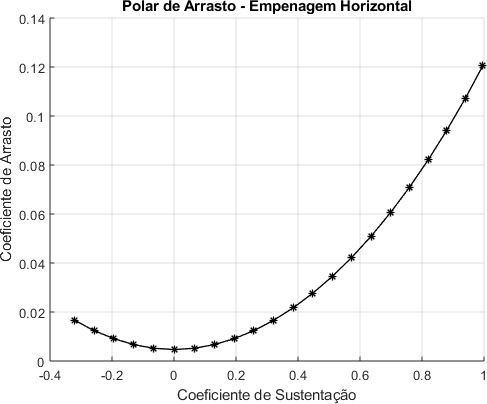
\includegraphics[width=0.75\textwidth]{images/parte3/eh_cl_cd.png}
\caption[Polar de arrasto para a Empenagem Horizontal]{Polar de arrasto para a Empenagem Horizontal}
\label{fig:eh_cl_cd}
\end{figure}

\begin{table}[H]
\centering
\begin{tabular}{cc}
\toprule
$ \frac{\partial C_{l}}{\partial \alpha} $ & 4.721 \\ [0.3cm]
$ \frac{\partial C_{L}}{\partial \alpha} $ & 3.567 \\ [0.3cm]
$ C_{L_{max}} $ & 1.097 \\ [0.3cm]
$ \alpha_{estol} $ & 18\textdegree\ \\ [0.3cm]
\bottomrule
\end{tabular}
\caption[Resultados - Empenagem Horizontal]{Resultados - Empenagem Horizontal}
\label{tbl:resultados_eh}
\end{table}

\subsection{Empenagem Vertical}
\label{ev}

\begin{figure}[H]
\centering
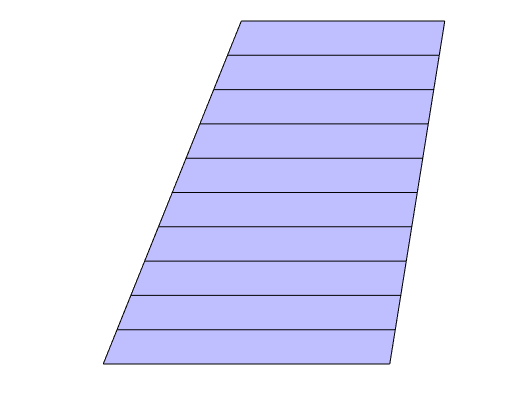
\includegraphics[width=0.45\textwidth]{images/parte3/malha_ev.PNG}
\caption[Paineis aerodinâmicos - Empenagem Vertical]{Paineis aerodinâmicos - Empenagem Vertical}
\label{fig:malha_ev}
\end{figure}

\begin{figure}[H]
\centering
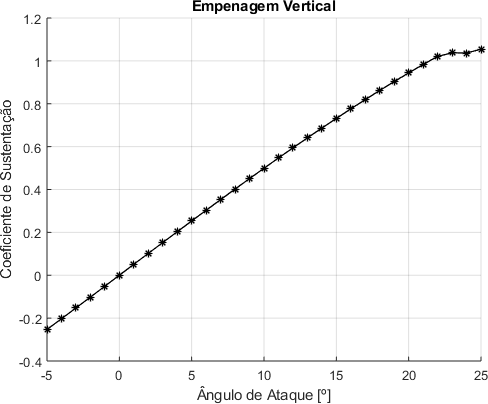
\includegraphics[width=0.75\textwidth]{images/parte3/ev_cl_alfa.png}
\caption[Curva $C_L$ x $\alpha$ para a Empenagem Vertical]{Curva $C_L$ x $\alpha$ para a Empenagem Vertical}
\label{fig:ev_cl_alfa}
\end{figure}

\begin{figure}[H]
\centering
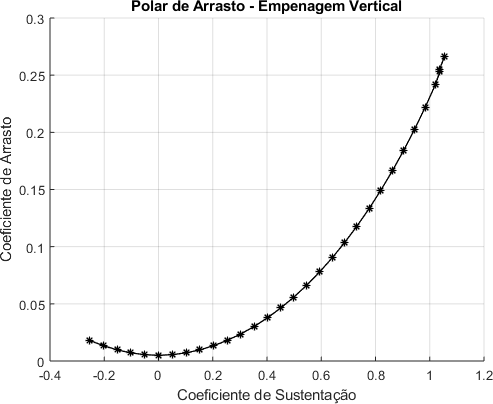
\includegraphics[width=0.75\textwidth]{images/parte3/ev_cl_cd.png}
\caption[Polar de arrasto para a Empenagem Vertical]{Polar de arrasto para a Empenagem Vertical}
\label{fig:ev_cl_cd}
\end{figure}


\begin{table}[H]
\centering
\begin{tabular}{cc}
\toprule
$ \frac{\partial C_{l}}{\partial \alpha} $ & 4.721 \\ [0.3cm]
$ \frac{\partial C_{L}}{\partial \alpha} $ & 2.630 \\ [0.3cm]
$ C_{L_{max}} $ & 1.054 \\ [0.3cm]
$ \alpha_{estol} $ & 23\textdegree\ \\ [0.3cm]
\bottomrule
\end{tabular}
\caption[Resultados - Empenagem Vertical]{Resultados - Empenagem Vertical}
\label{tbl:resultados_ev}
\end{table}
